\documentclass[../DS03.tex]{subfiles}%
\graphicspath{{./figures/}}%

\begin{document}
\section[29]"E"{RLC échelon montant}

\enonce{%
	\begin{tcn}[cnt, bld](impo)<lftt>{}
		Indiquer la ou les bonnes réponses en justifiant tout votre raisonnement.
	\end{tcn}

	On considère un circuit RLC série, alimenté par une source idéale de tension de
	force électromotrice $E$ constante comme schématisé ci-contre. Le condensateur
	peut être court-circuité lorsque l'interrupteur $K$ est fermé. On note $i(t)$
	l'intensité du courant qui traverse la bobine et $u_C(t)$ la tension aux bornes
	du condensateur C.

	\begin{figure}[htbp]
		\centering
		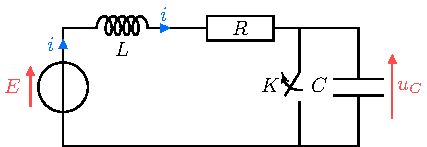
\includegraphics[width=.5\linewidth]{rlc_montant_switch}
	\end{figure}

	Le condensateur est mis en court-circuit par un interrupteur $K$ depuis une durée
	suffisamment longue, pour que le régime permanent soit établi. À l'instant pris
	comme origine des temps, on ouvre l'interrupteur $K$.
}%

\QR[5]{\label{q:1}%
	Que valent l'intensité $i\left(0^+\right)$ et la tension $u_C(0^+)$ à
	l'instant $t=0^+$, succédant immédiatement à l'ouverture de l'interrupteur $K$~?
	Justifier tout votre raisonnement.
	\begin{tasks}[label=\protect\fbox{\Alph*}, label-width=4ex](4)
		\task $i\left(0^+\right)=0$
		\task $i\left(0^+\right)=\frac{E}{R}$
		\task $u_C\left(0^+\right)=0$
		\task $u_C\left(0^+\right)=E$
	\end{tasks}%
}{\label{q:1}%
	Intéressons-nous d'abord au circuit à $t<0$. L'interrupteur est alors fermé si
	bien que $u_C$ est une tension aux bornes d'un fil donc
	\[
		u_C\left(t=0^-\right) = 0 \pt{1}
	\]
	De plus, le condensateur assure la continuité de la tension à ses bornes,
	donc
	\[
		u_C\left(t=0^+\right)=u_C\left(t=0^-\right)=0 \pt{1}
	\]
	Par ailleurs en régime permanent constant, on sait que la bobine est
	équivalente à un interrupteur fermé (un fil) \pt{1}. Si bien que le circuit est alors
	équivalent à uniquement la résistance $R$ en série avec la source idéale de
	fem $E$. Ainsi avec une loi des mailles et loi d'\textsc{Ohm}~:
	\[
		i\left(t=0^-\right)=E/R \pt{1}
	\]
	De plus, la bobine assure la continuité de l'intensité qui la traverse, donc
	\[
		i\left(t=0^+\right)=i\left(t=0^-\right)=\frac{E}{R} \pt{1}
	\]
	Réponses \fbox{B} et \fbox{C}.
}

\QR[6]{%
	Établir l'équation différentielle vérifiée par $u_C(t)$ pour $t>0$. On la
	mettra sous forme canonique en introduisant la pulsation propre $\w_0$ et le
	facteur de qualité $Q$~:
	\[
		\dv[2]{u_C}{t} + \frac{\w_0}{Q} \dv{u_C}{t} + \w_0{}^2 u_C(t) = \alpha
	\]
	Exprimer $\w_0$ et $Q$.
	\begin{tasks}[label=\protect\fbox{\Alph*}, label-width=4ex](4)
		\task $\w_0=\frac{1}{\sqrt{LC}}$
		\task $\w_0=\frac{1}{LC}$
		\task $Q=R\sqrt{\frac{L}{C}}$
		\task $Q=\frac{1}{R}\sqrt{\frac{L}{C}}$
	\end{tasks}
}{%
	On se place après l'ouverture de l'interrupteur ($t>0$). On a alors un circuit
	RLC série pour lequel on cherche à établir l'équation différentielle du second
	ordre sur la variable $u_C(t)$. Appliquons la loi des mailles en notant $u_R$
	et $u_L$ les tensions respectivement aux bornes du résistor et de la bobine.
	\smallbreak
	\begin{isd}
		\begin{DispWithArrows*}[fleqn, mathindent=2pt]
			u_L + u_R = u_C &\stm{=} E
			\Arrow{$u_L = L \dv{i}{t}$\\et $u_R = Ri$}
			\\\Lra
			L \dv{i}{t} + Ri + u_C &\stm{=} E
			\Arrow{$i = C \dv{u_C}{t}$}
			\\\Lra
			LC \dv[2]{u_C}{t} + RC \dv{u_C}{t} + u_C &\stm{=} E
			\Arrow{forme\\canonique}
			\\
			\Lra \dv[2]{u_C}{t} + \frac{R}{L} \dv{u_C}{t} + \frac{1}{LC}u_C &\stm{=}
			\frac{E}{LC}
		\end{DispWithArrows*}
		\tcblower
		Par identification, on a alors :
		\begin{gather*}
			{\w_0}^2 = \frac{1}{LC} \Lra \boxed{\w_0 \stm{=} \frac{1}{\sqrt{LC}}}
			\qMath{et}
			\frac{\w_0}{Q} = \frac{R}{L}
			\\\Lra
			Q = \frac{L\w_0}{R} = \frac{L}{R}\frac{1}{\sqrt{LC}}
			\Lra
			\boxed{Q \stm{=} \frac{1}{R}\sqrt{\frac{L}{C}}}
		\end{gather*}
		Réponses \fbox{A} et \fbox{D}.
	\end{isd}
}

\QR[1]{%
	Exprimer $\alpha$.
	\begin{tasks}[label=\protect\fbox{\Alph*}, label-width=4ex](4)
		\task $\alpha=0$
		\task $\alpha=E$
		\task $\alpha=QE$
		\task $\alpha= {\w_0}^2 \, E$
	\end{tasks}
}{%
	\leftcentersright{%
		En poursuivant l'identification~:
	}{%
		$\boxed{\alpha = \frac{E}{LC} \stm{=} {\w_0}^2E}$
	}{%
		Réponse \fbox{D}
	}%
}

\QR[2]{%
	Que peut-on affirmer concernant le facteur de qualité ?
	\begin{tasks}[label=\protect\fbox{\Alph*}, label-width=4ex]
		\task La durée du régime transitoire est la plus brève lorsque $Q=2$.
		\task La durée du régime transitoire est la plus brève lorsque $Q=1/2$.
		\task Plus la valeur de l'inductance est élevée, plus le facteur de qualité
		est faible.
		\task Plus la valeur de la capacité est élevée, plus le facteur de qualité
		est faible.
	\end{tasks}
}{%
	La durée du régime transitoire est la plus brève lorsque le système a une
	évolution pseudo-périodique avec un très faible dépassement, soit pour un
	$Q>1/2$ (précisément, c'est pour $Q=\num{0.72}$ \pt{1}). Aucune des deux
	premières réponses A ou B n'est juste. Notons en revanche que pour $Q=1/2$, on
	a le transitoire le plus bref sans dépassement. Par ailleurs, le facteur de
	qualité s'écrivant
	\[
		Q=\frac{1}{R}\sqrt{\frac{L}{C}}
	\]
	Une inductance élevée induira un facteur de qualité grand tandis qu'une
	capacité élevée conduira à un facteur de qualité petit. \pt{1}
	\medskip
	Réponse \fbox{D}.
}

\enonce{%
	Dans la suite, on considère que la bobine possède une inductance $L =
		\SI{50}{mH}$ et que la capacité du condensateur vaut $C =\SI{20}{\mu F}$. On
	souhaite obtenir un facteur de qualité $Q = 10$.
}%

\QR[2]{%
	Calculer la valeur à donner à la résistance $R$ du résistor.
	\begin{tasks}[label=\protect\fbox{\Alph*}, label-width=4ex](4)
		\task $R=\SI{0,002}{\ohm}$
		\task $R=\SI{0,02}{\ohm}$
		\task $R=\SI{5}{\ohm}$
		\task $R=\SI{500}{\ohm}$
	\end{tasks}
}{%
	On cherche la valeur de $R$ pour obtenir $Q=10$ à $L$ et $C$ fixé.
	On isole alors $R$ dans l'expression de $Q$~:
	\smallbreak
	\centersright{%
		$\DS\boxed{%
				R \stm{=} \frac{1}{Q}\sqrt{\frac{L}{C}}}
			\Ra
			\xul{R = \SI{5}{\ohm}
			} \pt{1}$
	}{%
		Réponse \fbox{C}.
	}%
}

\enonce{%
	On admet alors que la tension aux bornes du condensateur évolue selon :
	\[
		u_C(t) =
		\exp(- \frac{t}{\tau})
		\left[A\cos{\left(\Wt\right)+B\sin{\left(\Wt\right)}}\right] + u_{C,p}
	\]
}

\QR[6]{%
	Exprimer $\tau$ en fonction de $\w_0$ et $Q$. Justifier tout votre
	raisonnement.
	\begin{tasks}[label=\protect\fbox{\Alph*}, label-width=4ex](4)
		\task $\tau=\frac{\w_0}{2Q}$
		\task $\tau=\frac{2Q}{\w_0}$
		\task $\tau=\frac{\w_0}{Q}$
		\task $\tau=\frac{Q}{\w_0}$
	\end{tasks}
}{%
	Le polynôme caractéristique associé à l'équation différentielle canonique
	s'écrit~:
	\smallbreak
	\begin{isd}
		\vspace{-15pt}
		\begin{gather*}
			r^2+\frac{\w_0}{Q}r+{\w_0}^2 \stm{=} 0
			\\\Ra
			\Delta =
			\left(\frac{\w_0}{Q}\right)^2-4{\w_0}^2 \stm{=}
			{{\w}_0}^2\left(\frac{1}{Q^2}-4\right) \stm{<} 0
			\\\beforetext{car}
			Q = 10 > \frac{1}{2}
		\end{gather*}
		\tcblower
		\vspace{-15pt}
		\begin{gather*}
			\Ra
			r_\pm \stm{=}
			-\frac{\w_0}{2Q}\pm j \frac{\sqrt{-\Delta}}{2} =
			-\frac{\w_0}{2Q}\pm j \w_0 \sqrt{1-\frac{1}{4Q^2}}
			\intertext{%
				Que l'on identifie en cohérence avec $u_C\left(t\right)$~:
			}
			r_\pm \stm{=} -\frac{1}{\tau}\pm j\W
			\Lra
			\boxed{\tau \stm{=} \frac{2Q}{\w_0}}
		\end{gather*}
		Réponse \fbox{B}.
	\end{isd}
	\vspace{-15pt}
}

\QR[1]{%
	Exprimer la pseudo-pulsation $\W$ en fonction de $\w_0$ et $Q$. Justifier
	tout votre raisonnement.
	\begin{tasks}[label=\protect\fbox{\Alph*}, label-width=4ex,
			% item-indent=-1em,
			column-sep=4em](4)
		\task $\W=\w_0\sqrt{1-\frac{1}{4Q^2}}$
		\task $\W=\w_0\sqrt{\frac{1}{4Q^2 }-1}$
		\task $\W=\w_0\left(1+\frac{1}{4Q^2}\right)^{1/2}$
		\task $\W=\frac{\w_0}{\sqrt{1-\frac{1}{4Q^2}}}$
	\end{tasks}
}{%
	\leftcentersright{%
		De même, par identification,
	}{%
		$\DS\W = \frac{\sqrt{-\Delta}}{2} \stm{=} \w_0\sqrt{1-\frac{1}{4Q^2}}$
	}{%
		Réponse \fbox{A}.
	}%
}

\QR[1]{%
	Exprimer $u_{C,p}$ en fonction de $E$. Justifier tout votre raisonnement.
	\begin{tasks}[label=\protect\fbox{\Alph*}, label-width=4ex](4)
		\task $u_{C,p}=E$
		\task $u_{C,p}=0$
		\task $u_{C,p}=\w_0{}^2 E$
		\task $u_{C,p}=2E$
	\end{tasks}
}{%
	$u_{C,p}$ est la solution particulière de l'équation différentielle. On peut la
	chercher sous la forme d'une constante. Soit, en l'injectant dans l'équation
	différentielle~:
	\begin{gather*}
		\underbracket[1pt]{\dv[2]{u_{C,p}}{t}}_{=0} +
		\frac{\w_0}{Q} \underbracket[1pt]{\dv{u_{C,p}}{t}}_{=0} +
		\w_0{}^2 u_{C,p}(t) =
		\w_0{}^2 E
		\Lra
		\boxed{u_{C,p} \stm{=} E}
		\tag*{Réponse \fbox{A}}
	\end{gather*}
}

\QR[1]{%
	Exprimer A. Justifier tout votre raisonnement.
	\begin{tasks}[label=\protect\fbox{\Alph*}, label-width=4ex](4)
		\task $A=E$
		\task $A=-E$
		\task $A=0$
		\task $A=E/2$
	\end{tasks}
}{%
	Exprimons la constante d'intégration $A$ à l'aide des conditions initiales
	déterminées à la question~\ref{q:1}~:
	\smallbreak
	\centersright{%
		$u_C\left(t=0^+\right) =
			0 =
			\exp(-0/\tau)\left[A\cos{\left(0\right)}+B\sin{\left(0\right)}\right] + E
			\Lra
			\boxed{A \stm{=} -E}$
	}{%
		Réponse \fbox{B}.
	}%
}

\QR[5]{%
	Exprimer B. Justifier tout votre raisonnement.
	\begin{tasks}[label=\protect\fbox{\Alph*}, label-width=4ex,
			item-indent=2.5em, column-sep=4em](4)
		\task $B=\frac{E}{\W}\pa{\frac{1}{RC}-\frac{1}{\tau}}$
		\task $B=\frac{E}{{RC\w}_a}$
		\task $B=0$
		\task $B=\frac{E}{{\tau \w}_a}$
	\end{tasks}
}{%
	D'après~\ref{q:1} , on a aussi $i\left(t=0^+\right)=E/R$.
	Or, la loi courant tension aux bornes du condensateur permet d'écrire que~:
	\smallbreak
	\begin{isd}[sidebyside align=top]
		\begin{DispWithArrows*}[]
			\eval{\dv{u_C}{t}}_{0^+} = \frac{i\left(t=0^+\right)}{C} &\stm{=}
			\frac{E}{RC}
			\\\text{Or,}\qquad \qquad
			{\dv{u_C}{t}} &\stm{=}
			-\frac{1}{\tau}\exr^{-\frac{t}{\tau}}
			\left[A\cos(\Wt)+B\sin(\Wt)\right] \\
			&+
			\W\times \exr^{\frac{t}{\tau}}
			\left[-A\sin(\Wt)+B\cos(\Wt)\right]
			\\\Ra
			\eval{\dv{u_C}{t}}_{0^+} &\stm{=} -\frac{A}{\tau}+\W B=\frac{E}{RC}
		\end{DispWithArrows*}
		\tcblower
		\begin{DispWithArrows}[]
			\Lra
			\W B &= \frac{E}{RC}+\frac{A}{\tau}
			\notag
			\Arrow{$A = -E$}
			\\\Lra
			\Aboxed{B &\stm{=} \frac{E}{\W}\left(\frac{1}{RC}-\frac{1}{\tau}\right)}
			\tag*{Réponse A}
		\end{DispWithArrows}
		\vspace{-15pt}
		\begin{gather*}
			\beforetext{De plus,}
			\tau = \frac{2Q}{\w_0} = \frac{2}{R}\sqrt{\frac{L}{R}}\times\sqrt{LC}
			\Lra
			\boxed{\tau \stm{=} \frac{2L}{R}}
		\end{gather*}
	\end{isd}
	Donc $\tau$ ne s'exprime pas en fonction de $R$ et $C$ uniquement. Ainsi, la
	réponse B est fausse. De même, $RC$ ne peut pas s'exprimer simplement en
	fonction de $\tau$ donc la réponse D est fausse.
	% \vspace{-15pt}
}

\end{document}
